\documentclass{article}
\usepackage[brazil]{babel}
\usepackage[utf8]{inputenc}
\usepackage{amsmath}
\usepackage{Sweave} % O arquivo Sweave.sty deve estar presente

\begin{document}

\section{Um documento em Markdown}

\subsection{Sobre o Markdown}

O Markdown é uma linguagem de marcação muito simples, desenvolvida por
John Gruber.

A ideia básica por trás da linguagem é fazer com que o escritor se
preocupe mais com o \textbf{conteúdo} do texto do que com a
\emph{formatação}.

\subsection{Mais um título}

Aqui vamos tentar descrever uma análise.

\subsection{Simulando variáveis aleatórias}

No R podemos simular valores de uma distribuição normal padrão através
da função \texttt{rnorm()}.

Seja $X \sim \text{N}(0,1)$, então para gerar 30 valores dessa
variável aleatório normal, fazemos

\begin{Schunk}
\begin{Sinput}
> (x <- rnorm(30))
\end{Sinput}
\begin{Soutput}
 [1]  0.2666528  0.8346728 -0.9044872 -1.8580406  0.6094493  2.3475377
 [7] -0.1716590 -1.4546268 -0.3508387 -0.8704386 -0.5282742  0.4109944
[13] -1.1312329 -1.1982299  0.2123786 -0.3140455 -0.1301582  0.6446011
[19]  0.4124025  0.9299942  1.1117137  0.1863256  0.4041974 -0.6206467
[25] -1.1469357 -0.1137552 -0.3499753 -1.4061662 -0.8155502 -1.1988132
\end{Soutput}
\end{Schunk}

\subsection{Comentários}

Com o resultado dessa simulação, podemos calcular a média e a variância
dessa VA $X$ para conferir se o resultado fica próximo de 0 e 1,
respectivamente.

\subsection{Visualização}

Também podemos fazer um histograma dessa VA $X$ simulada

\begin{figure}
\begin{Schunk}
\begin{Sinput}
> hist(x)
\end{Sinput}
\end{Schunk}
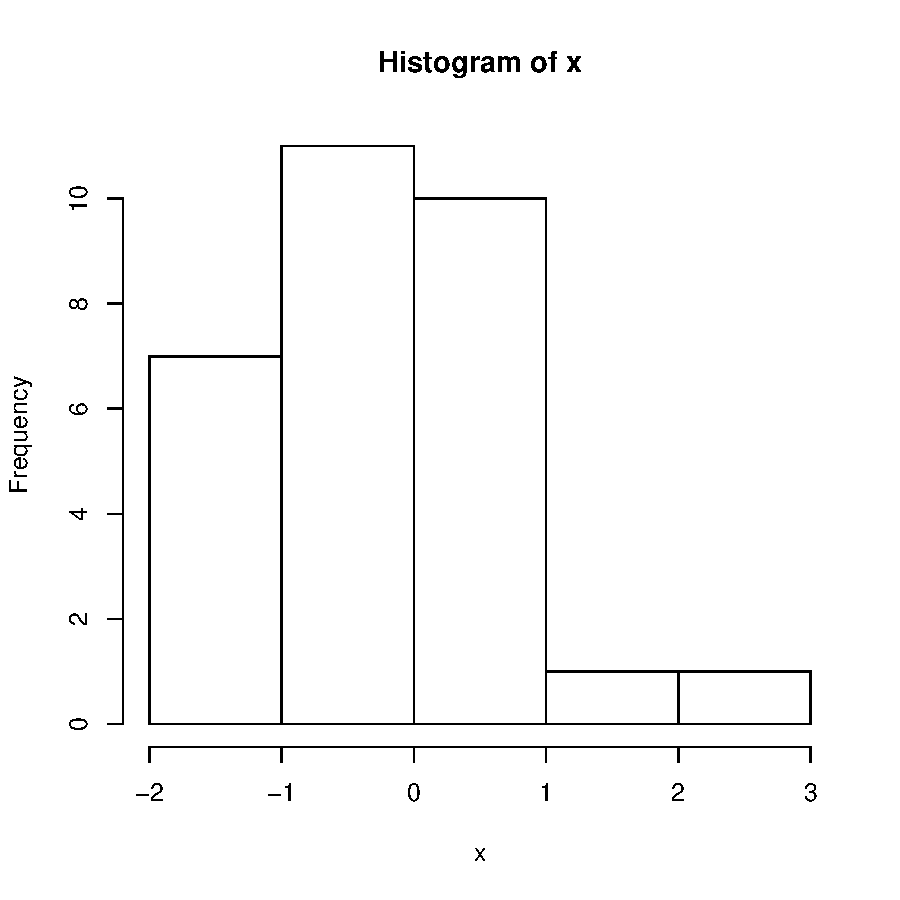
\includegraphics{Exemplo0-Sweave-histm}
\end{figure}

A média de $X$ é -0.206.

\end{document}
